
%%% Local Variables:
%%% mode: latex
%%% TeX-master: t
%%% End:

\chapter{基于多模态的入侵检测}
\label{cha:command}
本章节介绍如何使用Transformer在网络入侵领域进行多模态建模。Transformer最初被用于自然语言处理领域,由于其性能优越,因此被广泛应用于计算机视觉领域。随后人们发现了该架构在图像文本之间多模态建模能力。网络流量本身是一种模态,但对网络流量各种特征属性的描述以及其中的端口协议含义等属于另一种模态。数据集在给出数据的同时,会提供对该数据集的描述。对于传统的机器学习,该描述帮助研究者设计合理的数据预处理方法以及模型结构;对于深度学习模型,过去的研究者仅使用该描述确定预处理方法,特别是哪些属性应该被设置独热编码,以及确定模型的输入维度。

过去的研究都没有充分利用数据及描述信息,这主要是因为缺少合适的模型(Transformer)结构以及使用该结构进行多模态建模的正确方法(CLIP\cite{pmlr-v139-radford21a})。本章根据最新的研究进展,提出了一种多模态入侵检测模型,该模型将数据及描述信息融入分类过程中,实现文本辅助建模,并根据实验验证本章提出方法的有效性。

\section{相关技术介绍}
\subsection{Transformer模型介绍}
Transformer的出现在深度学习领域是变革性的,该模型在2017年被提出,作为性能卓越的自然语言处理的工具。该模型最大的特点在于其使用自注意力机制(Self-Attention)处理时序数据,这与之前主流的RNN或CNN模型截然不同。

使用自注意力机制进行建模,带来了以下优点:

\begin{enumerate}
    \item 自注意力机制能够捕获长距离相关信息且不会出现信息衰减,主流的RNN存在长距离信息衰减问题,CNN则只能建模局部信息。
    \item 自注意力机制并行处理序列信息,而RNN则是顺序处理,并行处理在一定程度上克服了访存限制对模型推理或训练速度的影响。
    \item 自注意力本质上是通过序列之间的相关性计算权重,即权重是动态的,而CNN等传统方法其权重值由模型本身决定是静态的。动态加权为模型提供了更高的灵活性和通用性。
\end{enumerate}

Transformer模型的结构由两部分组成:编码器以及解码器,如\ref{fig:transformer_struct}图示。

\begin{figure}[htbp]
    \centering
    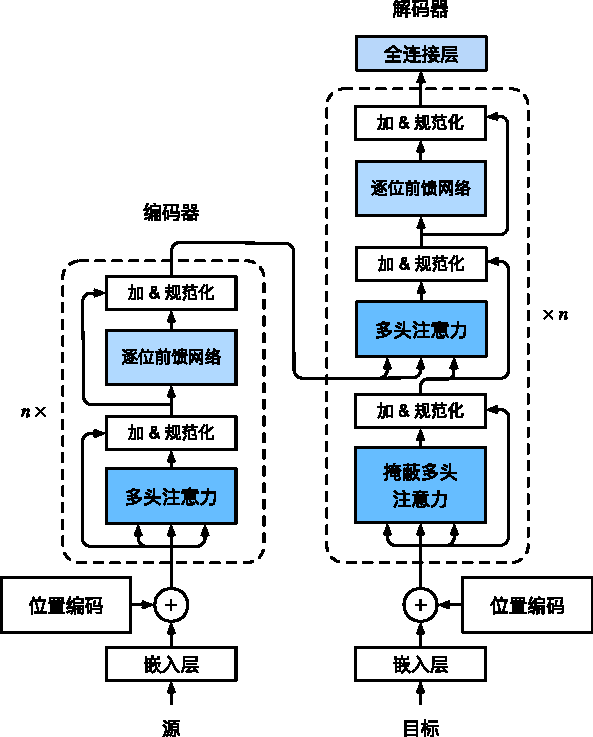
\includegraphics[width=.67\linewidth]{img/multimodal/transformer.pdf}
    \caption{Transformer架构\cite{zhang2023dive}}
    \label{fig:transformer_struct}
\end{figure}

左侧为编码器,编码器由多个相同的层组成,每一层中有两个子层,第一个子层是多头注意力,第二个子层是前馈网络。每个层在输出时都会进行层归一化以及残差连接。

右侧是解码器,同样由多层组成,每一层包含三个子层,增加的第三个子层用于接收编码器输入,在每一层的最下侧子层增加了掩码,用于保证信息由过去位置流向未来位置。

\subsection{BERT模型介绍}
BERT(Bidirectional Encoder Representations from Transformers),是一种基于Transformer架构的自然语言模型,关键特征在于双向,即在训练过程中同时考虑输入左侧以及右侧的全部上下文。传统的RNN只能进行单向建模,叠加两层不同方向的RNN才能实现双向建模。

BERT具有强大的自然语言理解能力,能感知句子中词语的深刻含义及不同词语之间的关系。该模型通过文本预训练进行学习,分别是掩码语言建模(Masked Language Modeling, MLM)和下一句预测(Next Sentence Prediction, NSP),前者遮挡词语并使用模型预测遮挡的内容,后者选取两句话,使用模型判断两句话是否存在上下文关系。经过预训练后,BERT只需在下游任务如句子情感分析等任务上进行微调即可取得较好性能。

对于每个输入序列,BERT模型都会将特殊的词语[CLS]对应的向量加入序列的开头。该向量在设计之初,用于捕捉整个输入序列的全局信息,在序列级别下游任务中该向量通常作为整个序列的特征。经典的序列集任务如句子情感分类,通常使用[CLS]作为输入,通过分类器得到最终分类结果。

\subsection{多模态模型介绍}
CLIP(Contrastive Language–Image Pre-training)是由OpenAI开发的多模态模型,其通过大量的图像-文本对进行训练,从而理解图像与自然语言之间的关系。其特点如下:
\begin{enumerate}
    \item 该模型通过对比学习进行训练,因此可完成多模态检索任务。通过文本检索图像,可在许多数据集上实现零样本图像分类。
    \item 该模型使用的文本编码器与图像编码器都基于Transformer架构,即通过同一架构的不同形式,可将文本与图像映射至同一特征空间中。
\end{enumerate}

CLIP由两部分组成,分别是图像编码器与文本编码器,如图\ref{fig:clip_struct}示。两者分别负责图像与文本的输入,并将其转化为统一空间中的向量表示。通过计算余弦相似度得到两向量之间的相似程度,在训练过程中是同一图像文本对之间的编码相互接近,而不同图像-文本对之间的编码相互远离。

\begin{figure}[htbp]
    \centering
    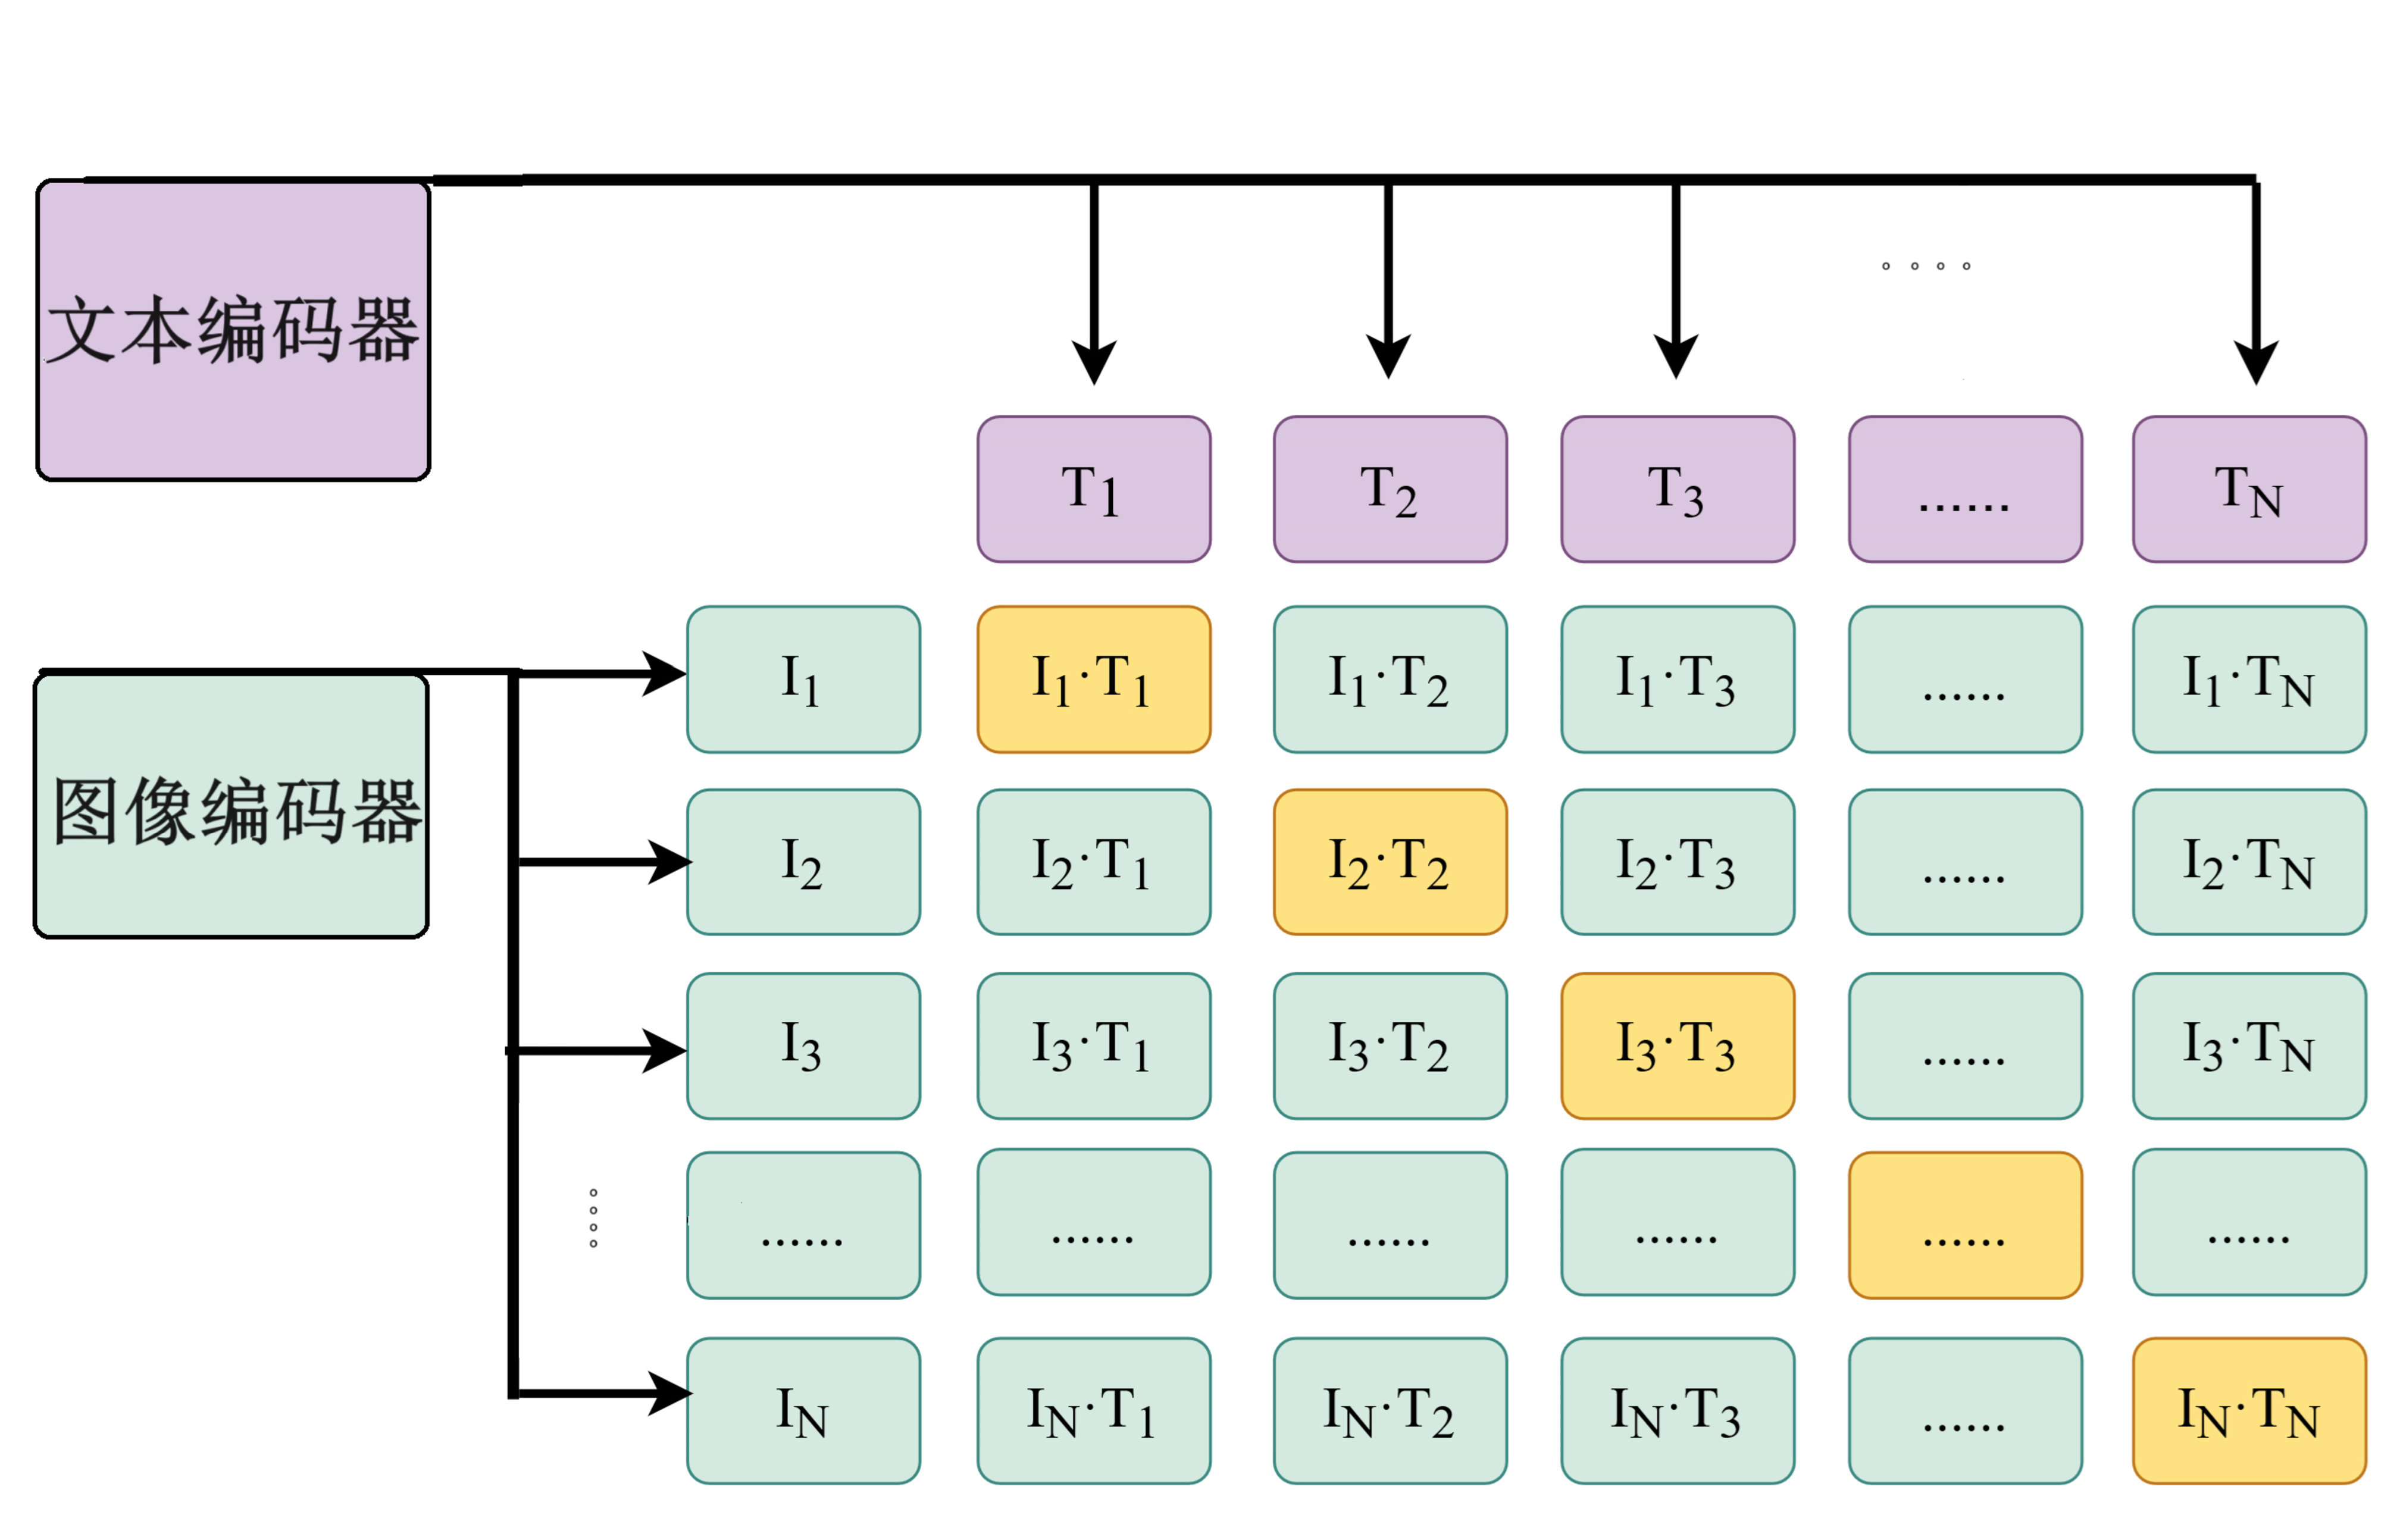
\includegraphics[width=1\linewidth]{img/multimodal/clip-overview.pdf}
    \caption{CLIP架构}
    \label{fig:clip_struct}
\end{figure}

CLIP模型的提出在多模态学习领域具有里程碑的意义,即通过大规模预训练模型可有效结合不同模态之间的信息,且两种编码器在本质上是同构的,Transformer架构在多模态学习中有极强的潜力。

\section{模型总体结构}

\begin{figure}[htbp]
    \centering
    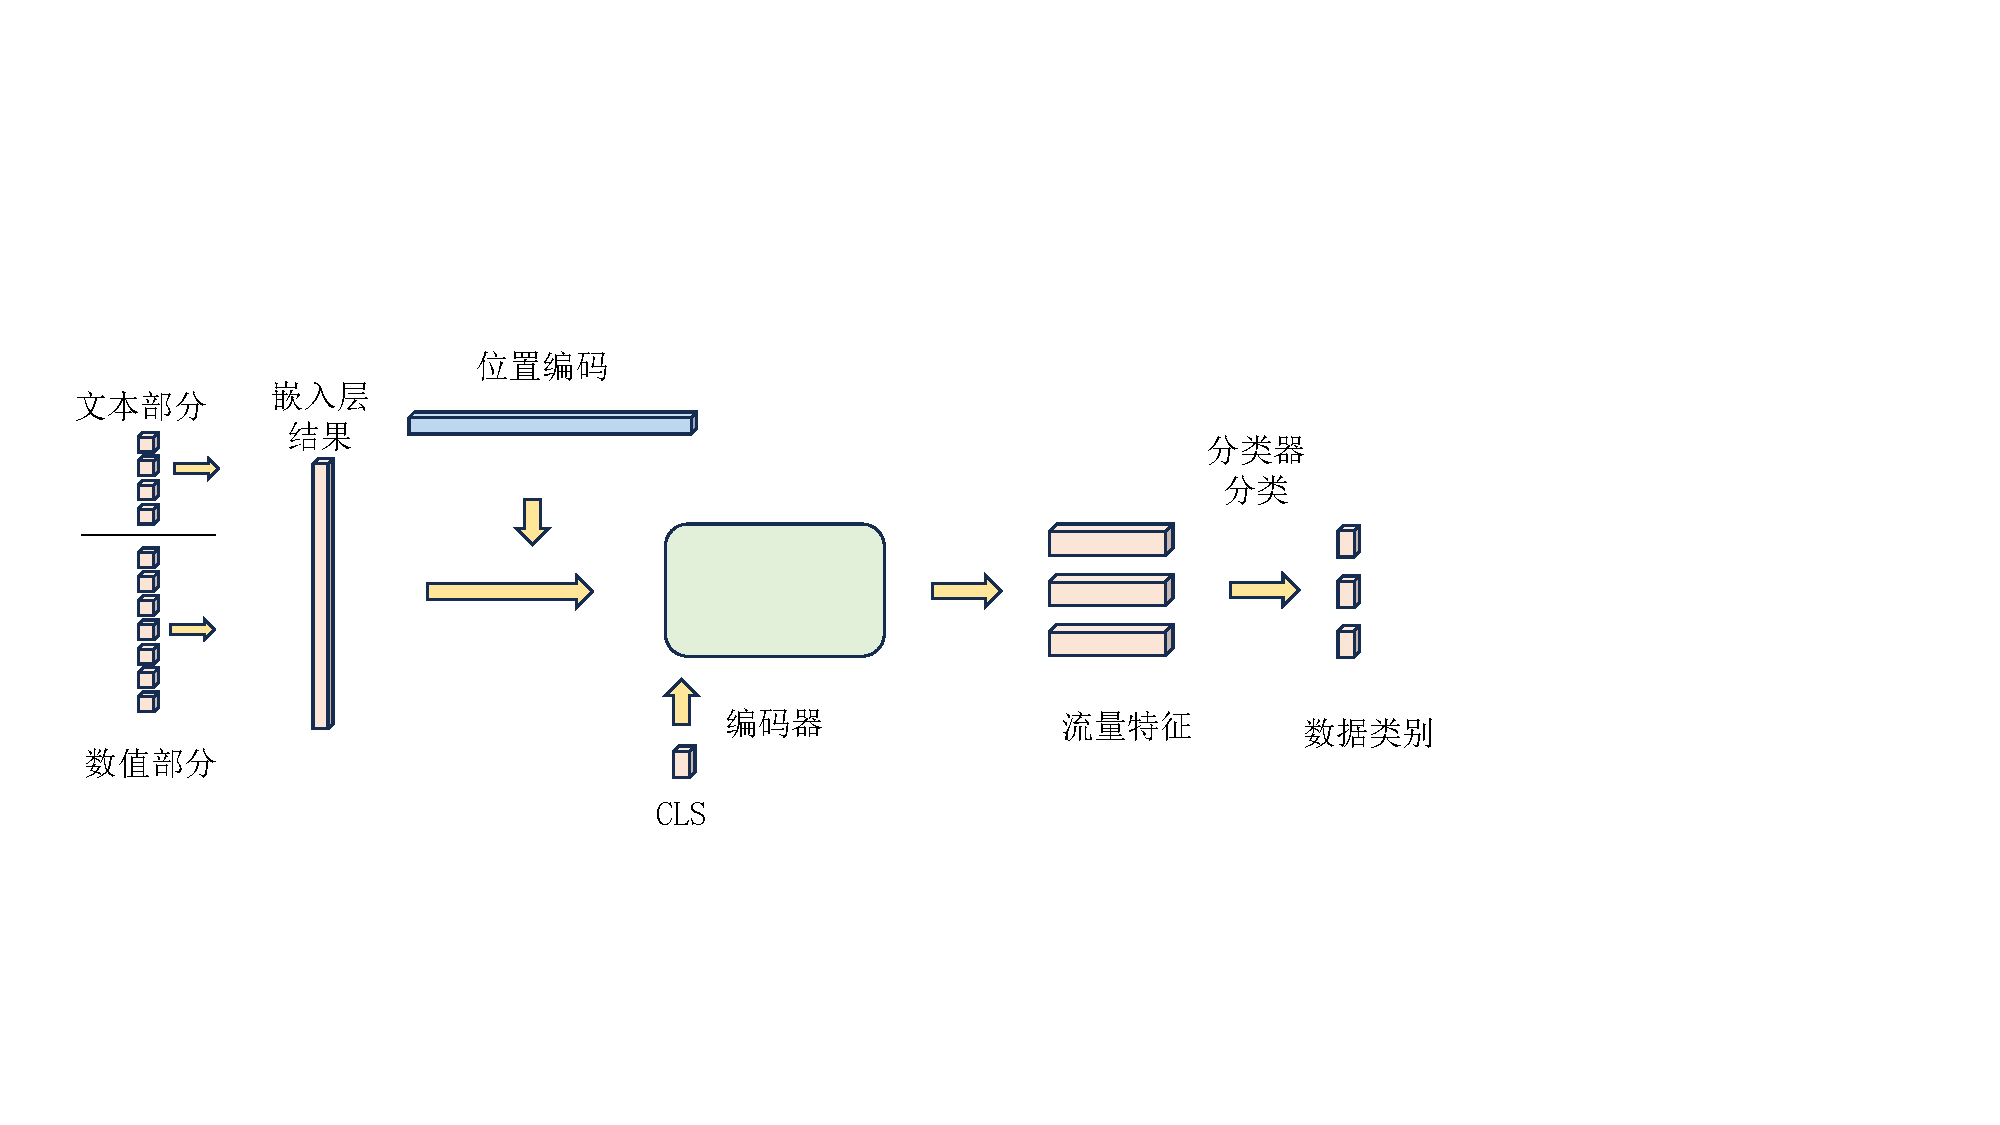
\includegraphics[width=1\linewidth]{img/multimodal/simple_overview.pdf}
    \caption{模型总体结构}
    \label{fig:simple_overview}
\end{figure}

本章提出的模型总体结构如图\ref{fig:simple_overview}示,其中左侧部分为语义辅助建模,是本章提出的多模态入侵检测模型的关键部分,其中包含新的数值嵌入方法、BERT加全连接层的文本嵌入方法以及数据集描述生成的位置编码。模型的输入是一个网络流量数据包的初步分析特征以及每个特征对应的文本描述。特征中包含多个属性,每个属性可以是数值类型或文本类型,若为文本则以索引形式给出。模型根据输入的特征判断数据包所属类别。模型由三个部分组成:嵌入层与位置编码、Transformer 编码器和分类器,Transformer 编码器由自注意力机制、归一化以及前馈神经网络组成。

在嵌入层,网络流量数据的初步分析特征 $\mathbf{X} = (\mathbf{x}_1, \mathbf{x}_2, \ldots, \mathbf{x}_n)$ 会进行变换以适应Transformer 编码器的输入特点。对于每个属性 $\mathbf{x}_i$,根据其模态分成两部分进行处理,最终得到128维的向量编码。在位置编码阶段,根据每个特征对应的文本描述生成位置编码。通过以上两个阶段,可得到了融合了属性值信息和属性描述信息的输入表示 $\mathbf{X}^{\mathrm{mm}} = (\mathbf{x}_1^{\mathrm{mm}}, \mathbf{x}_2^{\mathrm{mm}}, \ldots, \mathbf{x}_n^{\mathrm{mm}})$,其中
$$
\mathbf{x}_i^{\mathrm{mm}} = \mathbf{v}_i^{\mathrm{word}} + \mathbf{v}_i^{\mathrm{desc}}
$$
这里 $\mathbf{v}_i^{\mathrm{word}}$ 表示第 $i$ 个属性值的嵌入向量,可以是 $\mathbf{v}_i^{\mathrm{num}}$ 或 $\mathbf{v}_i^{\mathrm{text}}$。

随后将得到的输入表示 $\mathbf{X}^{\mathrm{mm}}$ 输入到4层的Transformer 编码器中。输入之前在序列的开头添加一个特殊的“[CLS]”标记,用于表示全局信息及整个数据包的特征,该标记的参数是可学习的。设第 $l$ 层Transformer Encoder的输出为 $\mathbf{Z}^{(l)} = (\mathbf{z}_0^{(l)}, \mathbf{z}_1^{(l)}, \ldots, \mathbf{z}_n^{(l)})$,其中 $\mathbf{z}_0^{(l)}$ 表示“[CLS]”标记对应的输出,$\mathbf{z}_i^{(l)}$ 表示第 $i$ 个属性的输出。最终得到第四层Transformer Encoder的“[CLS]”标记对应的输出,即输出的 $\mathbf{z}_0^{(4)}$ 作为整个数据包的表征向量。最后在分类阶段使用softmax函数将 $\mathbf{z}_0^{(4)}$映射到每个类别的概率。

\section{模型单层结构}

\subsection{语义辅助建模简介}
\begin{figure}[htbp]
    \centering
    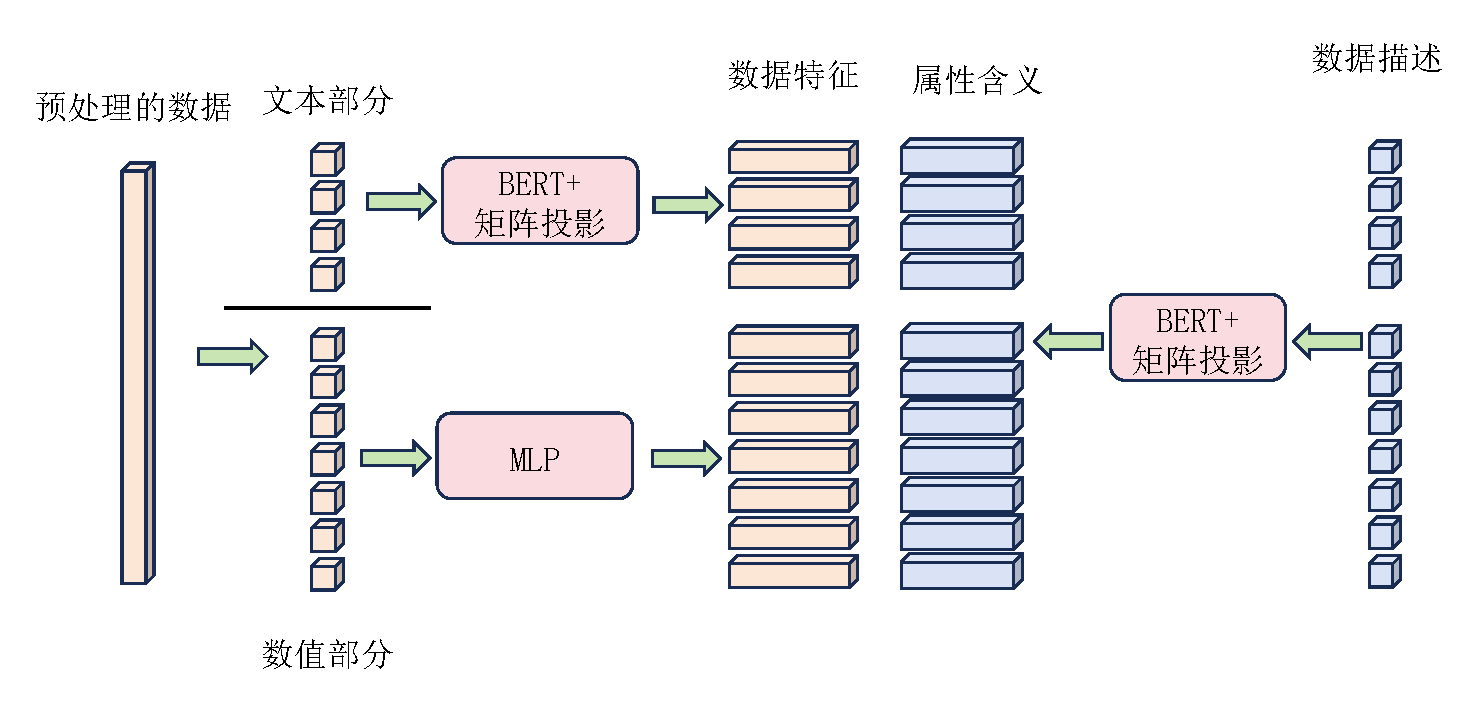
\includegraphics[width=\textwidth,height=\textheight,keepaspectratio]{img/multimodal/data2vec.pdf}
    \caption{获取嵌入向量及位置编码}
    \label{fig:data2vec}
\end{figure}

语义辅助建模包含两个过程数据嵌入以及位置编码,如图\ref{fig:data2vec}示,数据嵌入由两种嵌入方法组成,位置编码由数据集中对数据的描述文本生成,这两步是实现多模态模型的核心步骤。

嵌入层将输入数据转化为模型能处理的向量。嵌入的设计是多模态模型的关键部分,多模态模型必须处理与整合来自不同模态的信息,每种模态的格式各异。为有效融合来自各个模态的数据,对每种模态设计合适的向量嵌入方法,通过向量嵌入,不同模态的信息可在同一向量空间中表示。

Transformer核心特点是无状态,传统RNN在处理序列时会保留内部状态以跟踪序列的位置信息。Transformer感知位置关系的核心在于位置编码。对于多模态模型,位置编码的设计是核心,编码显式地提供了位置信息,位置信息可以是实际的前后关系,也可以是抽象位置(逻辑位置)如是否是文本以及是否是图像。序列中的每个元素加入位置编码后,除了包含其自身信息,还包含其所在位置信息。对于多模态模型,位置编码帮助模型识别元素的模态。

本章使用语言模型生成位置编码,为序列中每个元素提供灵活的位置信息;同时使用两种嵌入机制,将文本与数值均映射为128维向量。模型通过上述过程可有效分析来自文本与来自数值的信息,为单个流量生成更准确的向量描述。

总体过程如下:
输入序列 $ \mathbf{X} = (\mathbf{x}_1, \mathbf{x}_2, \ldots, \mathbf{x}_m) $中每个元素 $\mathbf{x}_i$ 是一个向量,向量的每个维度可能是数值或文字,总维度是$n$,与输入序列描述的个数相同。输入序列对应的描述 $ \mathbf{Desc} = (\mathbf{desc}_1, \mathbf{desc}_2, \ldots, \mathbf{desc}_n) $,对于序列中的每个元素 $\mathbf{x}_i$,执行以下步骤:

\begin{enumerate}
    \item 将 $\mathbf{x}_i$ 分离成数值部分 $\mathbf{n}_i$ 和文字部分 $\mathbf{t}_i$。
    \item 对数值部分 $\mathbf{n}_i$ 中的每个数值应用多层感知机 ${\mathrm{MLP}}_1$,得到数值的表征向量 $\mathbf{v}_i^{\mathrm{num}}$:
    \begin{equation}
    \mathbf{v}_i^{\mathrm{num}} = {\mathrm{MLP}}_1(\mathbf{n}_i)
    \end{equation}
    \item 使用BERT中获取文本部分 $\mathbf{t}_i$ 对应的句子表征向量 $\mathbf{w}_i$,然后应用线性投影 ${\mathrm{Proj}}_1$,得到文字的表征向量 $\mathbf{v}_i^{\mathrm{text}}$:
    \begin{equation}
    \mathbf{w}_i = {\mathrm{BERT}}(\mathbf{t}_i)
    \end{equation}
    \begin{equation}
    \mathbf{v}_i^{\mathrm{text}} = {\mathrm{Proj}}_1(\mathbf{w}_i)
    \end{equation}
    \item 对 $\mathbf{x}_i$ 向量中对应的描述$\mathbf{desc}_i$ ,从使用BERT获得对应的句子表征向量 $\mathbf{d}_i$,然后应用线性投影 ${\mathrm{Proj}}_2$,得到描述的表征向量 $\mathbf{v}_i^{\mathrm{desc}}$:
    \begin{equation}
    \mathbf{d}_i = {\mathrm{BERT}}(\mathbf{desc}_i)
    \end{equation}
    \begin{equation}
    \mathbf{v}_i^{\mathrm{desc}} = {\mathrm{Proj}}_2(\mathbf{d}_i)
    \end{equation}
    
\end{enumerate}

最终,对于每个元素 $\mathbf{x}_i$,可得数值表征向量 $\mathbf{v}_i^{\mathrm{num}}$或文字表征向量 $\mathbf{v}_i^{\mathrm{text}}$,以及用于位置编码的描述表征向量 $\mathbf{v}_i^{\mathrm{desc}}$。对于前两种表征向量,按照其位置统称为 $\mathbf{v}_i^{\mathrm{word}}$。

经过语言辅助建模后输入序列 $ \mathbf{X}$变为了$ \mathbf{X}^{\mathrm{mm}} = (\mathbf{x}_1^{\mathrm{mm}}, \mathbf{x}_2^{\mathrm{mm}}, \ldots, \mathbf{x}_n^{\mathrm{mm}}) $,其中${x}_i^{\mathrm{mm}}$由以下方式得到:
    \begin{equation}
    \mathbf{x}_i^{\mathrm{mm}} = \mathbf{v}_i^{\mathrm{word}} + \mathbf{v}_i^{\mathrm{desc}}
    \end{equation}
   
后续只要将这些输入传统的Transformer模型,就可以实现对网络流量的建模。经过若干层变换后提取[CLS]即可得到固定维度为$d$的特征,该特征理论上与数据集无关,与流量本身的特点有关。

\subsection{嵌入层}
基于Transformer架构的模型在输入的第一步进行数据嵌入,该过程对数据进行处理,将信息转化为描述其含义的向量,方便模型对数据进行分析与特征提取。

面向自然语言处理的模型常采用的方法是词向量嵌入,即首先从文本数据中识别唯一单词建立词表,随后为每个词分配一个向量,每次都会根据查表结果替换为对应的向量,该向量会在随后的训练过程中进行调整。使用词向量可使在语义上含义相近的词在高倍空间其相对距离更近,因此词向量可有效表达每个词的复杂含义。与稀疏的独热编码相比,词向量是密集的,可有效节约存储空间。

面向计算机视觉的模型常采用的方法是图像切块,每个图像小块再进行线性映射或其他形式映射后,其表现形式与进行了词向量线路的单词相同,可进入Transformer架构中。

流量特征中包含许多文本信息如协议描述、所用端口的描述,这些文本已在数据处理过程中构建嵌入向量表并转化为索引值。传统方法将文本转换为独热编码,但这种方式会损失一部分文字的含义,且对端口号进行转换时,会生成非常稀疏的向量,不利于模型学习。

为了充分地体现文本之间的细微差异,重编码部分使用预训练BERT模型生成文本特征向量,从而得到文字对应的编码。具体方法是取[CLS]作为文本的向量表征。

理想情况下,将BERT嵌入到模型中并随着模型进行微调是最佳做法。然而,由于BERT的计算量较大,直接使用可能导致模型运行缓慢,无法实时监测流量情况。因此可将BERT视为参数固定的特征提取器,采用预计算加快模型计算速度。在数据预处理阶段,已经构建了句表,此表中包含可能用到的句子,预计算需要在模型初始化阶段,通过预训练的BERT系列中的“bert-large”生成句子对应的表征向量(维度1024)填充到句表中。在训练和推理阶段,模型可以直接使用处理后的特征结果,而无需运行完整的BERT模型。此方法既提高了效率,又能有效保留文字的语义信息。

以上过程可得到预计算的句子表征向量,所用的特征提取器BERT内部参数被冻结,即提取的嵌入向量表(句表)中向量并不会根据下游任务进行调整,为了针对网络入侵检测中的描述特征提取任务进行优化,需要为其增加可学习参数。另一方面,BERT得到的向量维度较高,对网络流量特征描述的句子较为简单,高维度向量中包含较多冗余,且影响计算速度。

因此需要引入参数可调节的矩阵进行投影,将句子表征向量从适应预训练任务的输出空间映射至适应入侵检测任务的空间。同时进行降维,以帮助模型适应流量检测的实时性要求。本节使用输入维度为1024,输出维度为128的线性变换进行投影,预计算后得到的嵌入向量表(句表)中的向量映射至合适的输出空间。

该设计可以把BERT模型和后面的投影看作整体,即规模较大且可以微调的语言模型。通常微调需要将数据经过BERT和线性投影变换进行前向传播,然后再反向传播经过线性投影变换,其中绝大多数计算量由BERT产生。

考虑到实际输入的文本是有限的,上述预计算过程已对可能输入的文本进行特征提取,因此可以将前向传播的第一步变为一种查表过程。此时微调就变成了查表过程加矩阵乘法的前向和反向传播过程,微调过程中矩阵投影的权重可在训练过程中调整,模型在较低计算量的情况下,仍保持学习能力。

Transformer输入序列的每一个向量维度都是相等的,此处输入序列的每一个元素指流量特征的每一个属性。网络流量特征中,大部分属性为数值类型,因此需将数值映射为句子表征向量,即将1024维数值映射为128维。此处使用简单的MLP实现数值映射,输入维度为1,隐藏层为512,输出维度为128,激活函数使用ReLU,引入该函数可增强模型非线性表示能力。此处MLP的隐藏层与输出维度参照Transformer中MLP进行设计,隐藏层与输出维度之比为2:1。

网络流量特征经过上述两个过程,每个属性值都转化为维度相同的向量。
\subsection{位置编码}
位置编码是Transformer架构的重要组成部分。在传统RNN模型,模型以递归方式按顺序处理输入序列,输入过程本身已包含位置信息。Transformer并行处理输入序列,序列中每个向量在形式上等价,若不进行位置编码,则模型无法区分向量在序列中的顺序。

Transformer架构解决这一问题的方法是引入位置编码。位置编码为模型提供显式的顺序信息,其具体方法是将与位置有关的向量添加到输入序列的每个元素中。原始Transformer使用余弦编码。

余弦位置编码基于三角函数构建,位置编码由定义好的函数计算得出,而不是模型在学习过程中得到。序列各处的位置编码维度与嵌入后的向量维度相同,但内容并不相同。对于位置 $pos$ 以及维度 $i$,在序列中位置编码 $\mathbf{PE}_{(pos, i)}$ 由公式\ref{eq:pe_cosine}定义。

\begin{equation}
\begin{aligned}
\mathbf{PE}_{(pos, 2i)} &= \sin\left(\frac{pos}{10000^{\frac{2i}{d}}}\right) \\
\mathbf{PE}_{(pos, 2i+1)} &= \cos\left(\frac{pos}{10000^{\frac{2i}{d}}}\right) \\
\end{aligned}
\label{eq:pe_cosine}
\end{equation}

其中 $pos$ 是序列中的位置,$i$ 是维度下标, $d$ 是信息编码后的维度。除固定的位置编码外,模型可在学习过程中调整位置编码,这被称为可学习位置编码。

可学习位置编码是模型用来学习序列中位置信息的一种参数。与预定义的余弦位置编码不同,可学习位置编码是模型参数的一部分,在模型训练中通过梯度下降进行调整。可学习位置编码 $\mathbf{E}_{pos}$ 由公式\ref{eq:Epos}定义。

\begin{equation}
\label{eq:Epos}
\mathbf{E}_{pos} = \{\mathbf{e}_{1}, \mathbf{e}_{2}, \ldots, \mathbf{e}_{N}\}
\end{equation}


其中 $N$ 是序列中的最大长度, $\mathbf{e}_{i}$ 是序列中第 $i$ 个位置的可学习位置编码。

在训练过程中模型会调整 $e_{i}$ 以最小化损失函数,虽然其长度相比余弦位置编码有一定限制,但其对特定任务的适应性更好。

在本章提出的模型中,位置编码需要对流量特征的每个属性提供信息。此位置的特点是,位置与其在输入序列中的相对位置并没有关系,而是与其对应的描述有关。通常情况下各位置的描述是固定的,因此可使用上述两种编码为模型提供属性描述信息。这种编码缺少灵活性,若新数据集中属性增加或删减,原有的位置编码可能会失效。

为解决上述两种编码在网络入侵检测任务上的局限性,本节提出一种新的语义辅助位置编码。该编码保持灵活性且通过引入语义信息实现对流量特征的更准确提取。与常规位置编码不同,此处的语义辅助位置编码并不是指的向量中每个元素在序列中的排列位置,而指的是每一个元素所对应的含义。此含义由数据集的每一列标题给出。

数据集的描述中会对每一列进行具体的介绍,说明其含义以及取值范围。因此可以使用预训练语言模型,如BERT,根据介绍文本生成每一列位置编码,其中包含每一列的含义。
BERT输入向量的维度较高,且原输出向量仅适合预训练任务,并不适合位置编码任务,位置编码相比之前的文本嵌入句子多样性更少,高维度向量会引入冗余信息,同样需要进行调整以实现降维处理。本节使用可学习的投影矩阵实现这一目的,使用投影矩阵将BERT生成的列标题描述向量转投影至适合位置编码的向量空间。

对于每个标题描述对应的[CLS]使用一个输入维度为1024,输出维度为128的矩阵变换实现,该矩阵是可学习的。经过变换,标题描述向量被映射到新空间。在此过程中BERT作为参数固定的特征提取器,[CLS]通过预计算得出,因此每次计算位置编码都只需对每个标题描述向量进行矩阵投影即可。这使模型能在实时计算的同时,有效利用数据集中对每一列的描述信息建立位置编码,以便模型对流量进行更精确建模。上述过程保持了模型的通用性,当数据集的格式发生变化,只需重新配置每一列的描述文本,再使用BERT进行一次推理,即可得到新的位置编码,不需要重新训练生成。

\subsection{自注意力机制}
自注意力机制是Transformer模型最大的特点,该过程本质上实现了对数据的自适应加权,过程可分为三个阶段。

第一步,使用三个投影矩阵$\mathbf{W}^{\mathrm{Q}} ,\mathbf{W}^{\mathrm{K}},\mathbf{W}^{\mathrm{V}}$,对经过语义辅助建模的$ \mathbf{X}^{\mathrm{mm}}$进行线性变换,可得到输入对应的查询、键和值矩阵:
\begin{equation}
\mathbf{Q} = \mathbf{X}\mathbf{W}^{\mathrm{Q}}, \quad \mathbf{K} = \mathbf{X}\mathbf{W}^{\mathrm{K}}, \quad \mathbf{V} = \mathbf{X}\mathbf{W}^{\mathrm{V}}
\end{equation}
如图\ref{fig:attention_proj} 示,该过程将输入序列转化为三个维度相同序列,这三个序列分别被称为查询、键、值。生成三种不同的序列可帮助模型对不同位置元素之间的相关性进行建模,建模过程类似信息检索,三个序列的含义如下:
\begin{itemize}
    \item 查询(Q)代表当前元素对序列中其他元素的关注程度,在计算注意力时,主要用于与其他元素的键进行比较,以确定相关性的强度。
    \item 键(K)代表序列的特征,该特征用于匹配查询。在计算注意力时,该元素决定了对查询来源的影响程度。
    \item 值(V)包含每个元素的实际信息。该元素根据Q与K之间的相关性被加权,权重反映了序列中全部元素对当前元素的重要程度。
\end{itemize}

\begin{figure}[htbp]
    \centering
    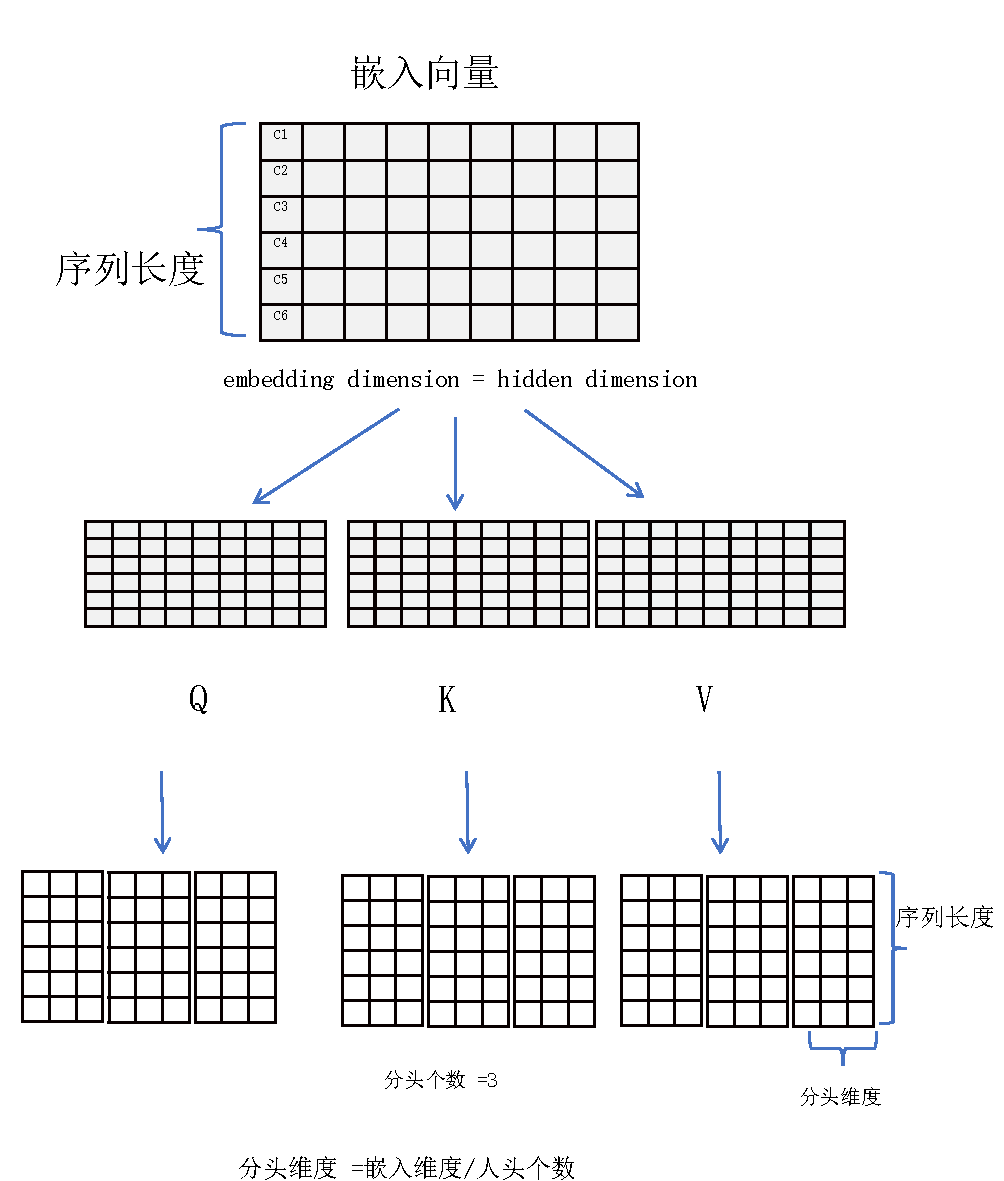
\includegraphics[width=0.85\linewidth]{img/multimodal/attention_proj.pdf}
    \caption{查询(Query)、键(Key)、值(Value)的生成}
    \label{fig:attention_proj}
\end{figure}

序列被划分为三个序列后,每个序列会被分成$h$个头,每个头对应的维度是${embedding\_dimension}/{h}$,此过程要求输入序列的维度必须被$h$整除。通过引入多个头,每个头都可以独立学到不同的注意力,即可以关注序列中的不同部分,而不是关注全局相关性,有助于模型捕捉更丰富的序列依赖关系。

每个头都可以独立计算注意力分数$\mathbf{Attention\_score}$,其中一个头的注意力计算分数如图\ref{fig:attention_softmax}示,将$\mathbf{Q}$与$\mathbf{K}$进行矩阵乘法,即对$\mathbf{Q}$的每一行以及$\mathbf{K}$的每一列计算向量点积,点积表示两个向量的相似程度,右侧注意力矩阵中第i行第j列的含义是第i个字与第j个字在该头的注意力值。对于两个服从均值为0,方差为1的正态分布的向量进行点积,点积后的结果就是向量的维度大小。因此在计算注意力分数时,需要在点积后,进行缩放,除以$\sqrt{d}$  ,将方差调整为1,避免高维度向量计算得出大数值,而导致梯度消失或爆炸。最后为保证某一元素对其他所有元素的注意力分数权值和为1,需要对最终的注意力分数按图\ref{fig:attention_softmax}中的行方向计算softmax。
\begin{figure}[htbp]
    \centering
    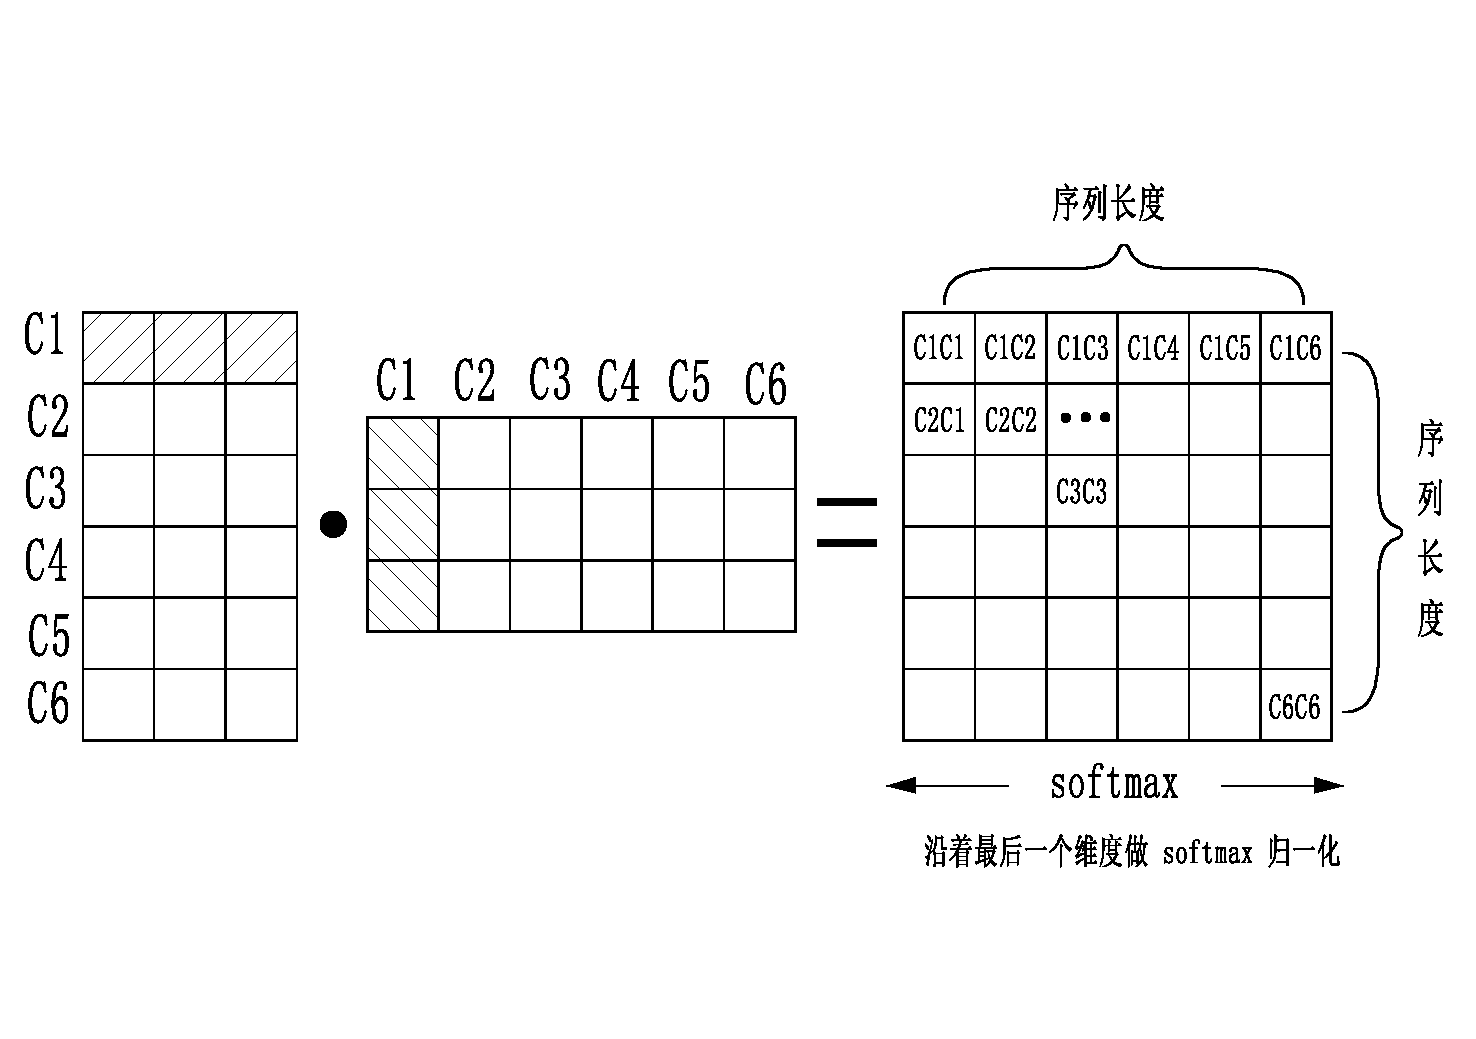
\includegraphics[width=0.8\linewidth]{img/multimodal/attention_softmax.pdf}
    \caption{注意力分数的计算 }
    \label{fig:attention_softmax}
\end{figure}
\begin{equation}
{\mathbf{Attention\_score}} = {\mathrm{softmax}}\left(\frac{\mathbf{Q}\mathbf{K}^{\mathrm{T}}}{\sqrt{d}}\right)
\end{equation}


最后在加权阶段,取每个头的注意力矩阵以及对应头的V,进行矩阵乘法如图\ref{fig:attention_fin}示。使用注意力权重对V进行加权,最终每个元素的值都包含了来自其他位置元素的信息。

\begin{equation}
{\mathbf{Attention}}=\mathbf{Attention\_score} \times \mathbf{V}= {\mathrm{softmax}}\left(\frac{\mathbf{Q}\mathbf{K}^T}{\sqrt{d}}\right)\mathbf{V}
\end{equation}

\begin{figure}
    \centering
    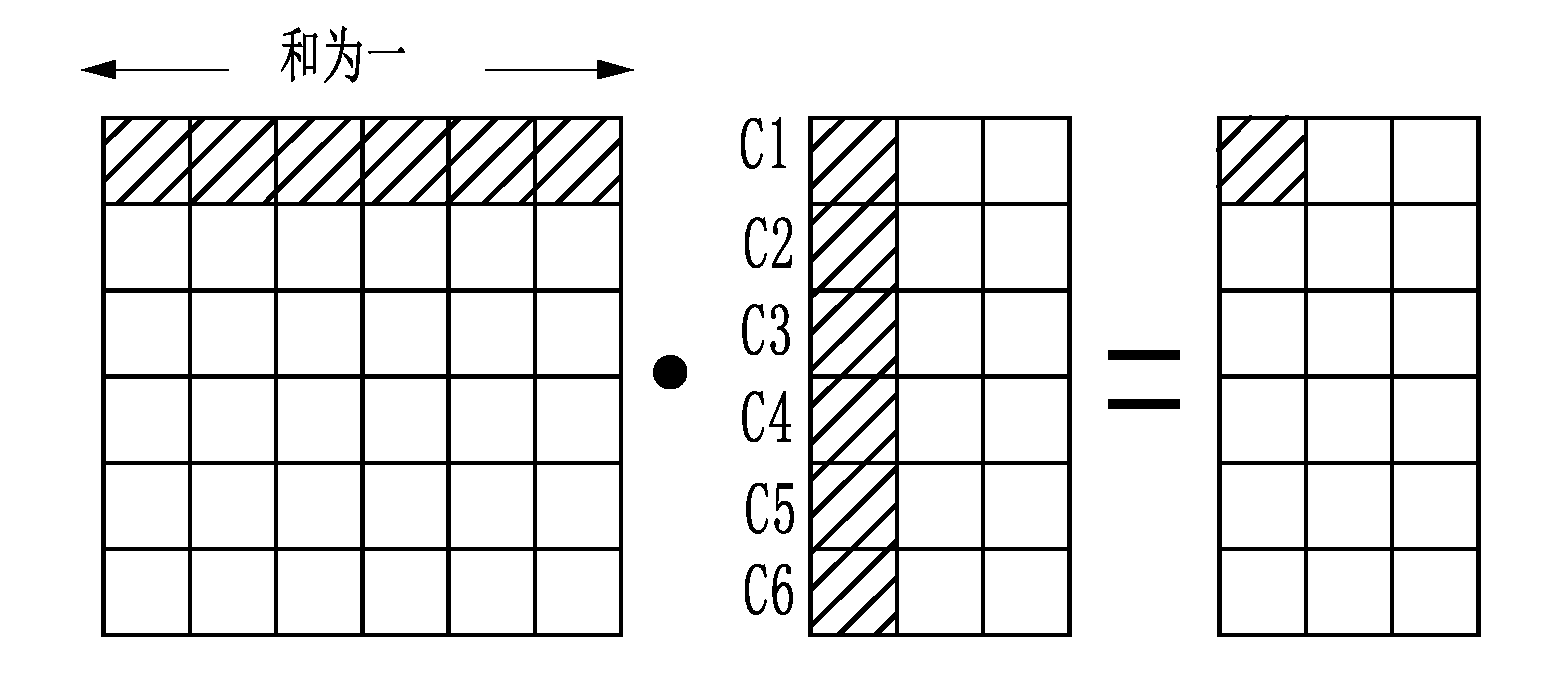
\includegraphics[width=0.8\linewidth]{img/multimodal/attention_fin.pdf}
    \caption{加权值向量的组合并生成输出 }
    \label{fig:attention_fin}
\end{figure}

\subsection{归一化}

在批次训练时有样本批次 $\mathbf{X} \in \mathbb{R}^{N \times D}$ ,其中 $N$ 是批次中样本的个数, $D$ 是隐藏层维度,对一个样本 $\mathbf{x} \in \mathbb{R}^D$, 可以计算均值 $\mu$ 以及方差 $\sigma^2$:

\begin{equation}
\mu = \frac{1}{D} \sum_{i=1}^{D} \mathbf{x}_i
\end{equation}

\begin{equation}
\sigma^2 = \frac{1}{D} \sum_{i=1}^{D} (\mathbf{x}_i - \mu)^2
\end{equation}


可以对输入每一个 $\mathbf{x}$ 归一化后的结果$\hat{\mathbf{x}}_i$:

\begin{equation}
\hat{\mathbf{x}}_i = \frac{\mathbf{x}_i - \mu}{\sqrt{\sigma^2 + \epsilon}}
\end{equation}

其中 $\epsilon$ 是一个小常量,用于避免除零错误。 然后归一化的 $\hat{x}$ 会被重新设置均值与方差以获得层归一化后的 $y$:

\begin{equation}
\mathbf{y}_i = \gamma \hat{\mathbf{x}}_i + \beta
\end{equation}

其中 $\gamma$ 和 $\beta$ 为输出需要被设置的方差与均值,这两个值均可随模型训练进行调整,因此模型可自适应调整每一层的输出分布,从而具有更灵活的特征提取能力。

\subsection{前馈神经网络}
Transformer 的前馈神经网络通常由MLP构成,其主要作用是增强模型的非线性表达能力。自注意力机制中都是线性变换,而前馈神经网络引入了非线性的激活函数,使模型能学到输入数据中的复杂关系,增强了模型对于信息的理解能力。该网络的作用是将自注意力机制生成的输出转化为新的特征表示。本章中使用的前馈神经网络结构如下:
\begin{equation}
\mathrm{FFN}(\mathbf{x})=\max(0, \mathbf{b_1} + \mathbf{W_1}\mathbf{x}) \mathbf{W_2} + \mathbf{b_2}
\end{equation}
其中$\mathbf{x}$是输入序列,$W_1\in \mathbb{R}^{d \times 2d}$和$W_2\in \mathbb{R}^{2d \times d}$是可学习的权重映射矩阵,$b_1 \in \mathbb{R}^{2d}$和$b_2\in \mathbb{R}^{d}$是偏置向量。
其过程有三步:
\begin{itemize}
\item 将输入值使用矩阵变换并加上偏置,该输入值被映射至两倍维度向量空间。
\item 对映射后的值,使用ReLU函数进行激活,即对映射后的向量,将负数部分置为0。
\item 将激活后的值使用矩阵变换并加上偏置,激活值被映射为与输入维度相同的向量空间。
\end{itemize}

\subsection{分类器}
模型的最后一步是进行分类。传统的分类方法是添加一个全连接层,通过线性映射得到各个类别对应的权重向量,即:

\begin{equation}
\mathbf{z} = \mathbf{W}\mathbf{x} + \mathbf{b}
\end{equation}

其中,$\mathbf{W}$ 是权重矩阵,$\mathbf{x}$ 是输入特征向量,$\mathbf{b}$ 是偏置向量。接着,通过计算softmax函数可以得到每个类别对应的概率:

\begin{equation}
P(\mathbf{y}_i|\mathbf{x}) = \frac{e^{\mathbf{z}_i}}{\sum_j e^{\mathbf{z}_j}} 
\end{equation}

\section{模型训练}

\subsection{损失函数}
损失函数用于评估模型性能,本章中使用的交叉熵损失函数评价模型的输出值与样本实际标签之间的差距大小,该函数在多分类问题中定义为:

\begin{equation}
L(\mathbf{y}, \mathbf{\hat{y}}) = -\sum_{c=1}^M y_{o,c} \log(\hat{y}_{o,c})
\end{equation}
其中 $M$ 是类别的总数,$y_{o,c}$ 是二进制指示器(0或1),表示类别 $c$ 是否是观察 $o$ 的正确分类,$\hat{y}_{o,c}$ 是模型预测观察 $o$ 为类别 $c$ 的概率。

入侵检测数据集呈现极度不均衡,为了解决这一问题可引入权重向量 $\mathbf{w}$,其中 $w_c$ 是与类别 $c$ 相关联的权重。改进后的加权交叉熵损失函数可以写为:

\begin{equation}
L(\mathbf{y}, \mathbf{\hat{y}}, \mathbf{w}) = -\sum_{c=1}^M w_c \cdot y_{o,c} \log(\hat{y}_{o,c})
\end{equation}
权重 $w_c$ 可以根据类别 $c$ 的样本频率来设置。为少样本类别设置更高的权重,可实现数据集的平衡,本章中各类别权重值为各类别频率的平方根倒数归一化后的结果。

模型对小样本类别误判后会得到更大程度调整使模型更注重该类别,从而减少模型在训练过程中对多数类别的偏好,最终在全部类别上都能有较高的分类准确率。

\subsection{优化器}
优化器调整模型参数,最小化损失函数,使模型预测更准确。本章使用AdamW优化器,为Adam(Adaptive Moment Estimation)的改进形式。Adam更新过程如下:

% 参数更新规则
\begin{equation}
\begin{aligned}
m_t &= \beta_1 \cdot m_{t-1} + (1 - \beta_1) \cdot g_t, \\
v_t &= \beta_2 \cdot v_{t-1} + (1 - \beta_2) \cdot g_t^2, \\
\hat{m}_t &= \frac{m_t}{1 - \beta_1^t}, \\
\hat{v}_t &= \frac{v_t}{1 - \beta_2^t}, \\
\theta_{t+1} &= \theta_t - \frac{\eta}{\sqrt{\hat{v}_t} + \epsilon} \cdot \hat{m}_t,
\end{aligned}
\end{equation}
其中 $g_t$ 是在时间步 $t$ 的梯度,$\beta_1$ 和 $\beta_2$ 是估计一阶矩(即均值)和二阶矩(即未中心化的方差)的指数衰减率,$\eta$ 是学习率,$\epsilon$ 是一个很小的常数,用来防止除以零。

AdamW对上述规则中的最后一项进行修改,改为:
\begin{equation}
\begin{aligned}
\theta_{t+1} &= \theta_t - \frac{\eta}{\sqrt{\hat{v}_t} + \epsilon} \cdot \hat{m}_t - \eta \cdot \lambda \cdot \theta_t,
\end{aligned}
\end{equation}
其中 $\lambda$ 是权重衰减系数。AdamW增加了一项 $- \eta \cdot \lambda \cdot \theta_t$,将权重衰减分离,使L2正则化更有效。


\section{实验设置与结果}

\subsection{评价指标}

入侵检测是多分类问题,对于每个类别有四种结果,如表\ref{base_classify_situation}示。
\begin{table}[!ht]
    \centering
    \caption{分类的情况}
    \label{base_classify_situation}
    \begin{tabular}{lll}
    \toprule
        ~ & 测试结果阳性 & 测试结果阴性 \\
    \midrule
        实际阳性(病例) & 真阳性(TP) & 假阴性(FN) \\
        实际阴性(非病例) & 假阳性(FP) & 真阴性(TN) \\
    \bottomrule
    \end{tabular}
\end{table}

这四种分类结果对每个类别衍生出了三种常见的评估指标,分别是召回率、精准率以及F1值,对于全部类别的综合指标则是正确率。召回率是该类别数据中被正确分类的比例,该值越高意味着对该类被漏报越少,对于类别$c$其定义如下:
\begin{equation}
{Recall}_c = \frac{TP_c}{TP_c + FN_c}
\end{equation}
精准率是被分成某一类中确实是该类的比例,该值越高意味着对该类别误报越少,对于类别$c$其定义如下:
\begin{equation}
{Precision}_c = \frac{TP_c}{TP_c + FP_c}
\end{equation}
F1值是上面两种数值的调和平均数,对于分布不均衡的数据集,F1值更能有效地体现分类器对某一类别的分类能力。

\begin{equation}
F1_c = 2 \cdot \frac{{Precision}_c \cdot {Recall}_c}{{Precision}_c + {Recall}_c}
\end{equation}


除单个类别的指标外,还有综合性指标准确率,该指标仅关注类别是否被正确分类,公式如下:
\begin{equation}
{ACC} = \sum_c\frac{TP_c+FN_c}{TP_c + TN_c + FP_c + FN_c}
\end{equation}

\subsection{实验设置}

根据本章提出的方法构建模型,使用AdamW作为优化器对模型参数进行调整。为了进一步提升模型训练效率,模型训练中引入了余弦退火调度策略,即根据事先设定的最小学习率和初始学习率自动调整学习率的大小。在训练的初始阶段还设置预热期,避免初始阶段模型参数急剧变化,导致模型不稳定。为确保可重复性,随机种子均设置为统一值。相关超参数如表\ref{tab:train_hyperargs}示。

\begin{table}[htb]
  \centering
  \caption{训练时的超参数设置}
    \begin{tabular}{ll}
    \toprule
\textbf{参数} & \textbf{值} \\
    \midrule
    优化器 & AdamW \\
    权重衰减(L2正则化项) & 0.0005 \\
    初始学习率 & 0.001 \\
    预热期初始学习率 & 0.000001 \\
    预热期持续周期 & 5  \\
    随机种子值 & 42 \\
    批量大小 & 4096 \\
    \bottomrule
    \end{tabular}
  \label{tab:train_hyperargs}
\end{table}

实验使用单个GPU下进行,为提升训练速度,同时减少显存消耗,实现效率和性能的最优平衡,实验中启用自动混合精度训练功能,实验平台如表\ref{tab:train_platform}示。

\begin{table}[htb]
  \centering
  \caption{实验平台}
    \begin{tabular}{ll}
    \toprule
\textbf{参数} & \textbf{值} \\
    \midrule
    操作系统 & windows10 22H2\\
    CPU & AMD AMD Ryzen 7 5800X \\
    GPU & GeForce RTX 4090 \\
    pytorch & 2.2.1 \\
    cuda & 12.1 \\
    \bottomrule
    \end{tabular}
  \label{tab:train_platform}
\end{table}

\subsection{实验结果}
本小节验证基于多模态入侵检测技术的核心,位置编码部分。本章介绍的位置编码有三种,分别是从数据集属性描述中生成的、使用公式\ref{eq:pe_cosine}生成的绝对位置编码,以及可学习的位置编码。

从表\ref{tab:exp_pe-tr-none}可看出,使用该编码器对网络流量进行编码,然后使用分类图进行分类,可得到99.63\% $\sim$ 99.66\%的准确率,其中使用三角函数进行绝对位置编码效果与使用文本生成的位置编码结果类似,仅相差3/10000,而使用可学习的位置编码效果表现最佳,准确率为99.66\%。以全部类别的总体准确率进行评价则三种位置编码的表现相似,三种位置编码并无显著区别。这三种分类模型对于样本数最少的未知攻击,攻击类型识别准确率为100\%,但f1分数值均小于0.6,说明模型对少类别样本识别标准较宽,因此能正确识别出全部少样本类别,但产生了较多误判,将其他类别的样本分入该类别。

\begin{table}[htb]
    \centering
    \caption{基于不同位置编码的通用编码器在CIC-IDS2017数据集上的表现}
    \begin{adjustbox}{max width=.535\textwidth}
    \begin{tabular}{lllll}
    \toprule
        编码形式 & 类别& 文本生成 & 余弦编码  &可学习\\ \midrule
        precision & BENIGN & 0.9995 & 0.9996 & \textbf{0.9996} \\
        precision & Web-Attacks & 0.6836 & 0.7463 & \textbf{0.8099} \\
        precision & Botnet & \textbf{0.4184} & 0.3813 & 0.3908 \\
        precision & PortScan & 0.9895 & \textbf{0.9911} & 0.9911 \\
        precision & Unknown & 0.28 & 0.1667 & \textbf{0.4118} \\
        precision & Denial-of-Service & 0.991 & \textbf{0.9914} & 0.9908 \\
        precision & Brute-force-attack & \textbf{0.9644} & 0.9378 & 0.9575 \\
        recall & BENIGN & 0.9962 & 0.9959 & \textbf{0.9962} \\
        recall & Web-Attacks & 0.9721 & 0.9708 & \textbf{0.9847} \\
        recall & Botnet & 0.9579 & \textbf{0.9652} & 0.9597 \\
        recall & PortScan & 0.9994 & \textbf{0.9995} & 0.9994 \\
        recall & Unknown & \textbf{1.0000} & \textbf{1.0000} & \textbf{1.0000} \\
        recall & Denial-of-Service & 0.9966 & 0.9981 & \textbf{0.9981} \\
        recall & Brute-force-attack & 0.9978 & \textbf{0.9965} & 0.9993 \\
        f1 & BENIGN & 0.9978 & 0.9978 & \textbf{0.9979} \\
        f1 & Web-Attacks & 0.8028 & 0.8438 & \textbf{0.8887} \\
        f1 & Botnet & \textbf{0.5824} & 0.5467 & 0.5554 \\
        f1 & PortScan & 0.9944 & \textbf{0.9953} & 0.9952 \\
        f1 & Unknown & 0.4375 & 0.2857 & \textbf{0.5833} \\
        f1 & Denial-of-Service & 0.9938 & \textbf{0.9947} & 0.9945 \\
        f1 & Brute-force-attack & \textbf{0.9808} & 0.9677 & 0.9779 \\
        acc& 全部& 0.9964 & 0.9964 & \textbf{0.9966} \\
    \bottomrule
    \end{tabular}
    \end{adjustbox}
    \label{tab:exp_pe-tr-none}
\end{table}

\begin{figure}[htbp] % 创建一个新的figure环境
\centering % 居中对齐所有的子图

\subfloat[文本生成位置编码]{ % 插入第二个子图及其标题
\begin{minipage}{0.45\linewidth}
\centering
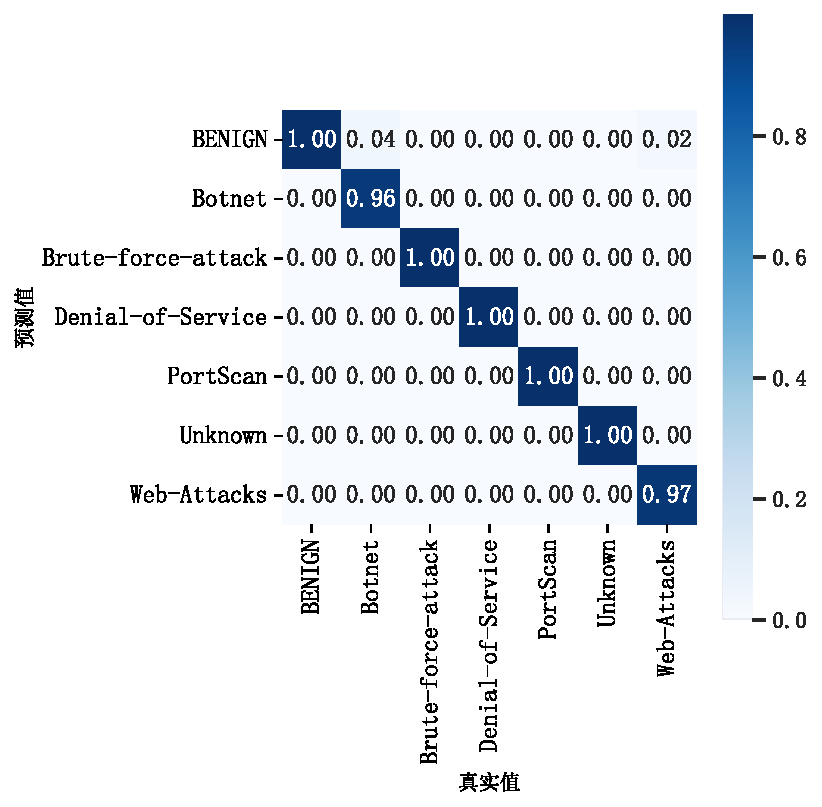
\includegraphics[width=1\linewidth]{img/exp1/4text-tr-none_confusion_matrix.pdf}
\label{fig:text-tr-none_cm}
\end{minipage}
}

\subfloat[绝对位置编码]{ % 插入第三个子图及其标题
\begin{minipage}{0.45\linewidth}
\centering
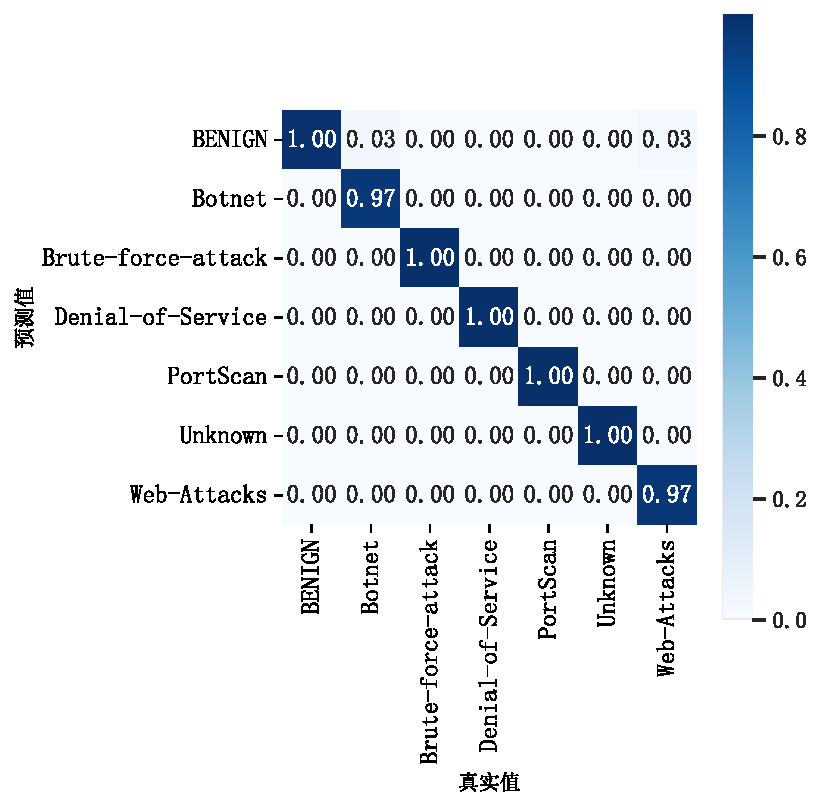
\includegraphics[width=1\linewidth]{img/exp1/5abs-tr-none_confusion_matrix.pdf}
\label{fig:abs-tr-none_cm}
\end{minipage}%
}
\subfloat[可学习位置编码]{ % 插入第四个子图及其标题
\begin{minipage}{0.45\linewidth}
\centering
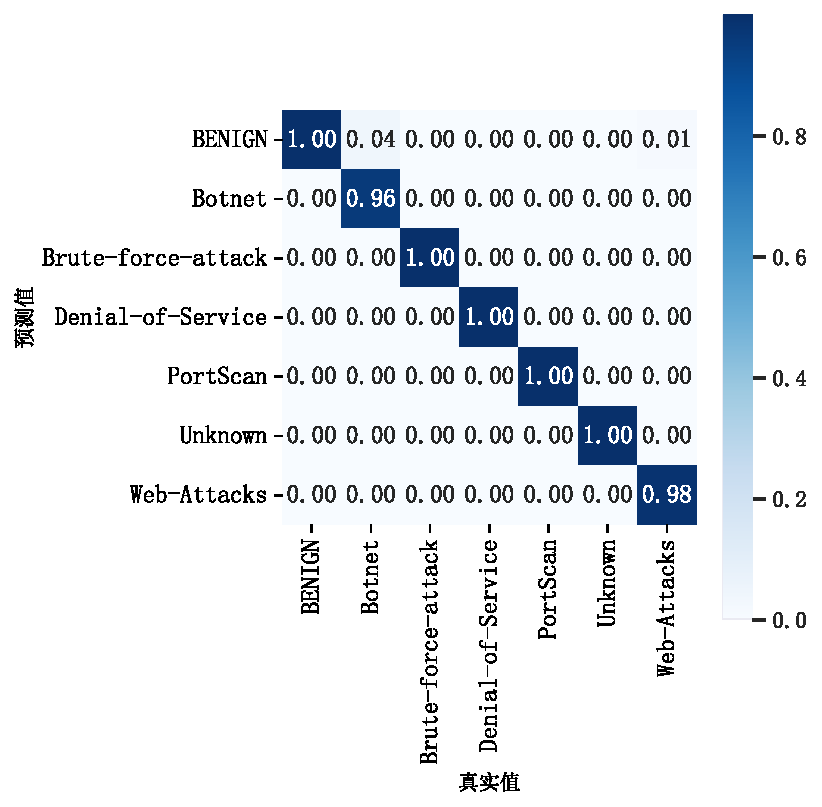
\includegraphics[width=1\linewidth]{img/exp1/6learned-tr-none_confusion_matrix.pdf}
\label{fig:learned-tr-none_cm}
\end{minipage}
}
\caption{基于不同位置编码模型的混淆矩阵} % 整个figure的标题
\label{fig:pe-tr-none_confusion_matrix}

\end{figure}

从混淆矩阵图\ref{fig:pe-tr-none_confusion_matrix}可看出分类模型对每一类样本的分类能力。这三种分类模型对于样本数量最多的4种类别(正常样本,端口扫描,拒绝服务,暴力攻击)达到了99\%以上的识别准确率。全部类别中三种模型对机器人网络流量的识别准确率均最低。

从以上的三个实验可看出,不同的位置编码对于非时序模型的影响较小,且使用文本生成的位置编码并无显著优势,反而总体准确率最低。这可能是因为生成的该编码本身性能较弱,也可能是受制于模型结构,该编码的性能并未完全展现。因此尽管本章并不对时序模型进行深入探讨,但为进一步验证不同时间编码的性能,以及为下一章内容进行预实验,会在这三种模型的基础上再加入4层Transformer进行时序建模实验。

\begin{table}[!ht]
    \centering
    \caption{增加时序Transformer后基于不同位置编码的通用编码器在CIC-IDS2017数据集上的表现}
    \begin{adjustbox}{max width=.75\textwidth}
    \begin{tabular}{lllll}
    \toprule
        编码形式 & ~ & 文本生成 & 余弦编码  &可学习  \\ \midrule
        precision & BENIGN & 0.9994  & 0.9994  & \textbf{0.9969} \\
        precision & Web-Attacks & \textbf{0.9071} & 0.6667  & 0.7000  \\
        precision & Botnet & \textbf{0.6729} & 0.4670  & 0.4904  \\
        precision & PortScan & 0.9942  & 0.9932  & \textbf{0.9947} \\
        precision & Unknown & 0.2500  & 0.1250  & \textbf{0.6205} \\
        precision & Denial-of-Service & \textbf{0.9986} & 0.9975  & 0.9982  \\
        precision & Brute-force-attack & \textbf{0.9267} & 0.7999  & 0.7758  \\
        recall & BENIGN & \textbf{0.9984} & 0.9962  & 0.9963  \\
        recall & Web-Attacks & \textbf{0.9791} & 0.9499  & 0.9652  \\
        recall & Botnet & \textbf{0.9908} & 0.9707  & 0.9835  \\
        recall & PortScan & 0.9956  & \textbf{0.9989} & 0.9968  \\
        recall & Unknown & \textbf{0.8571} & 0.7143  & 0.7143  \\
        recall & Denial-of-Service & 0.9987  & 0.9977  & \textbf{0.9994} \\
        recall & Brute-force-attack & 0.9964  & 0.9954  & \textbf{0.9968} \\
        f1 & BENIGN & \textbf{0.9989} & 0.9978  & 0.9980  \\
        f1 & Web-Attacks & \textbf{0.9417} & 0.7835  & 0.8115  \\
        f1 & Botnet & \textbf{0.8015} & 0.6306  & 0.6545  \\
        f1 & PortScan & 0.9949  & \textbf{0.9960} & 0.9957  \\
        f1 & Unknown & 0.3871  & 0.2128  & \textbf{0.6667} \\
        f1 & Denial-of-Service & 0.9987  & 0.9976  & \textbf{0.9988} \\
        f1 & Brute-force-attack & \textbf{0.9602} & 0.8870  & 0.8726  \\
        val/acc1 & all & \textbf{0.9983} & 0.9965  & 0.9968  \\
        \bottomrule
    \hline
    \end{tabular}
    \end{adjustbox}
    \label{tab:pe-tr-tr}
\end{table}

\begin{figure}[htbp] % 创建一个新的figure环境
\centering % 居中对齐所有的子图

\subfloat[文本生成位置编码]{ % 插入第二个子图及其标题
\begin{minipage}{0.5\linewidth}
\centering
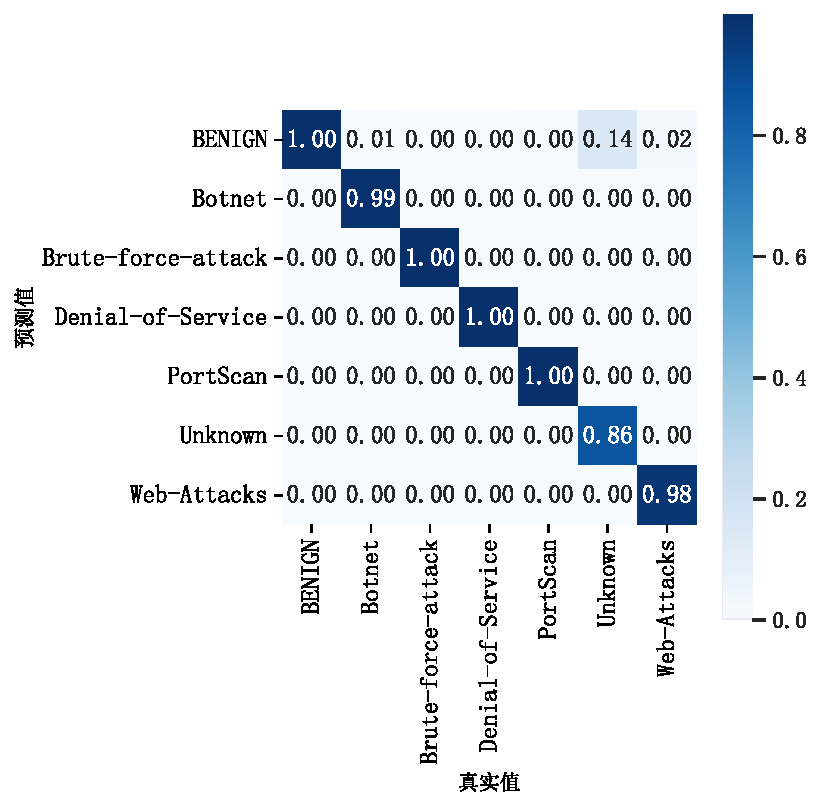
\includegraphics[width=1\linewidth]{img/exp1/1text-tr-tr_confusion_matrix.pdf}
\label{fig:1text-tr-tr_confusion_matrix}
\end{minipage}
}

\subfloat[绝对位置编码]{ % 插入第三个子图及其标题
\begin{minipage}{0.5\linewidth}
\centering
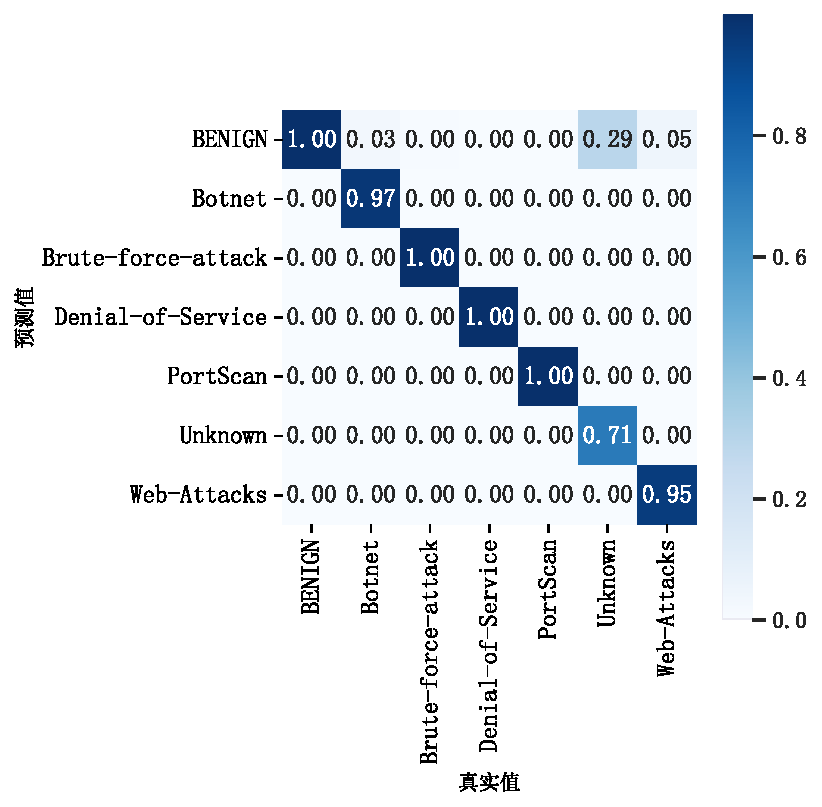
\includegraphics[width=1\linewidth]{img/exp1/2abs-tr-tr_confusion_matrix.pdf}
\label{fig:2abs-tr-tr_confusion_matrix}
\end{minipage}%
}
\subfloat[可学习位置编码]{ % 插入第四个子图及其标题
\begin{minipage}{0.5\linewidth}
\centering
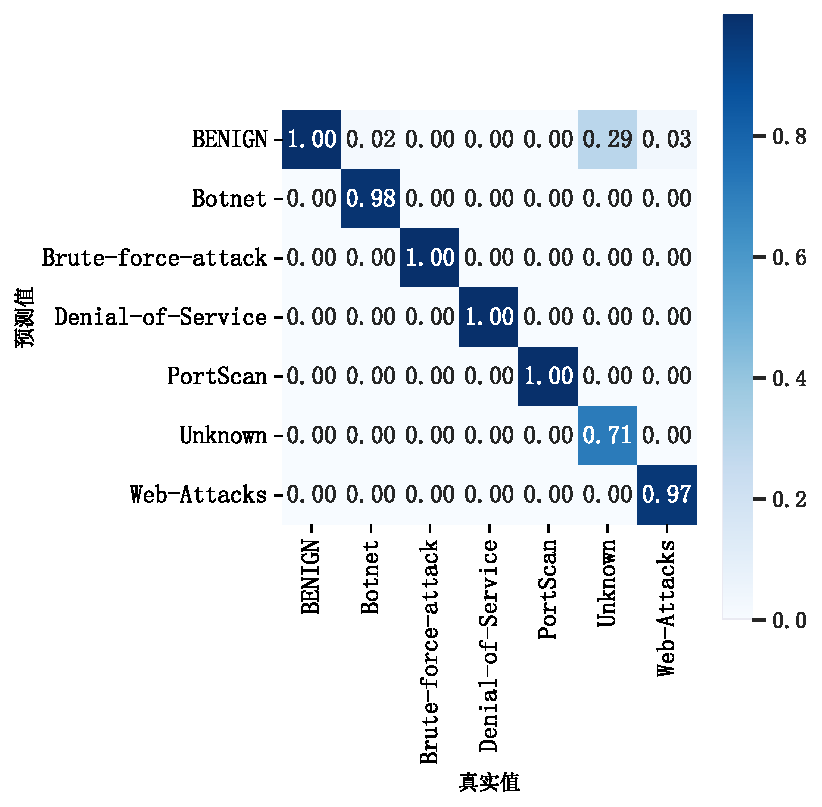
\includegraphics[width=1\linewidth]{img/exp1/3learned-tr-tr_confusion_matrix.pdf}
\label{fig:3learned-tr-tr_confusion_matrix}
\end{minipage}
}
\caption{增加时序Transformer后基于不同位置编码模型的混淆矩阵} 
\label{fig:pe-tr-tr_confusion_matrix}
\end{figure}

由表\ref{tab:pe-tr-tr}示,在通用编码器加时序模型的架构下,使用可学习位置编码以及绝对位置编码的两种模型,其识别准确率仍与原来架构相似,而使用文本生成的位置编码性能得到显著上升,综合准确率达到99.83\%。这说明使用基于文本生成的位置编码,有助于提升模型预测性能。如图\ref{fig:pe-tr-tr_confusion_matrix},从各小类的指标上分析,基于文本的位置编码在各小类别的数据表现性能上也显著优于可学习位置编码以及绝对位置编码。

\subsection{可视化分析}
位置编码为128维的向量,将不同位置的编码计算余弦相似度如图\ref{fig:pe_vis}示。从该图可看出,网络流量的第4个特征“Flow duration”与其他特征截然不同,相关度很低。位置编码沿对角线对称,相似语义的属性,其对应的位置编码也相似,如右下角,从第70个属性至最后一个属性均描述网络流量活动与空闲时间。从数据集的描述中可分析出相似的属性会被放置在相近的位置,但从该识别码可看出存在例外即数据特征的57-61维中,第59维‘Fwd Avg Bulk Rate’(前向方向的平均批量率) 与其他4个属性似乎关系较小,特别是之后的两个维度特征“后向方向的平均字节数批量率”和“后向方向的平均数据包批量率”,相差两个单词,后两维描述的方向与该特征不同,这说明网络流量具有单向性以及不对称性。

\begin{figure}[htbp]
    \centering
    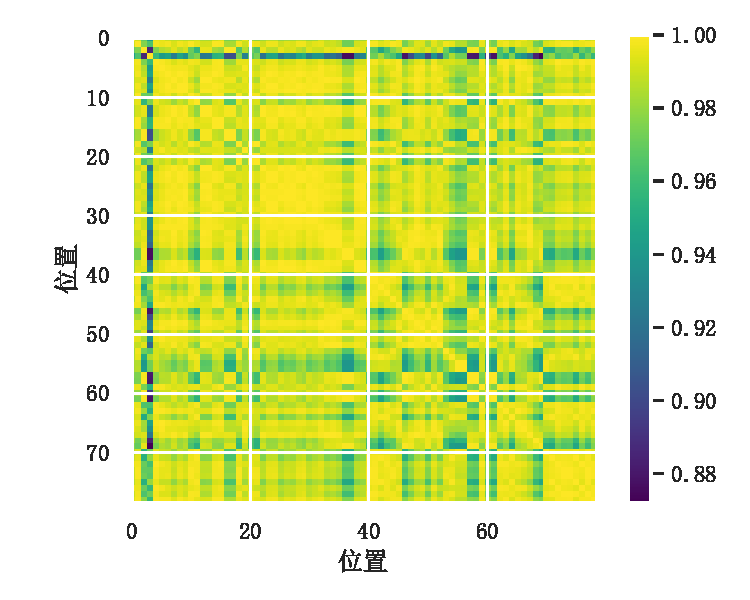
\includegraphics[width=0.75\linewidth]{img/multimodal/none-tr-tr-positional_encoding.pdf}
    \caption{位置编码可视化}
    \label{fig:pe_vis}
\end{figure}

\section{本章小结}

文章提出了一种基于多模态的入侵检测模型,该模型能有效融合网络流量属性值以及对该属性的描述信息,实现文本辅助建模。

在模型单层结构小节,重点介绍了语言辅助建模的两个关键步骤:重编码以及位置编码。前者将流量特征中的数值类型与文本类型映射为统一的128位向量,后者利用数据集中对属性的描述信息生成富含语义的位置编码,帮助模型识别每一个元素的具体含义。随后总结了语言辅助建模的整体过程,即将重编码后的结果与位置编码进行融合,从而得到输入Transformer编码器的向量。随后介绍了模型的其他组成部分,说明了各个部分的作用。

之后说明了模型的训练方法,及如何使用加权交叉熵函数实现不平衡样本的有效训练,以及如何使用AdamW 优化器进行参数更新。

最后通过实验证明了本章提出方法的有效性,最高可提升0.19\%的准确率,说明引入属性描述信息可以提高模型对网络流量建模的准确性。